% ============================================================
% ch3_dsp_background.tex
% ANSpect O-EMA · MS Thesis · UTD Electrical Engineering
% \input target — no \documentclass or \begin{document}
% STATUS: SKELETON — run 'expand CH-3.X' to flesh out
% v1.0  01-Sep-2026  Split from chapters.tex
% v1.1  01-Sep-2026  Corrections against ITU-T J.83 Annex B PDF ground truth:
%                    Fix: Transport framing — checksum replaces sync byte
%                         in every packet (not inverted every 8th)
%                    Fix: SRRC paragraph — removed non-standard impl params
%                         (span/sps/taps/output rate belong in CH-4)
%                    Fix: Trellis — BCC puncture rate 4/5 vs overall 19/20
%                    Fix: Gray coding claim flagged as unverified from std
%                    Fix: Table docsis_params — restored §B.6.1 info bit rate
%                    Fix: SRRC TODO — corrected citation key
%                    Fix: Trellis TODO — corrected rate description
% v1.2  01-Sep-2026  Removed \eqref{} from equation-introducing sentences
%                    in CH-3.3 — citation now on prose sentence only,
%                    \label{} retained for cross-reference
%                    Affected equations: eq:rs_primitive_poly,
%                    eq:rs_generator_poly, eq:rs_generator_expanded,
%                    eq:rs_message_poly, eq:rs_remainder,
%                    eq:rs_codeword, eq:rs_extended_symbol
% v1.3  02-Sep-2026  Replaced all bare acronyms with \ac{} commands
%                    per abbrevs.tex v1.2 scan results
%                    Removed manual (SHORT) expansions — glossaries handles
%                    first-use expansion automatically
%                    Flagged: duplicate sentence in RS subsection
%                    Flagged: RFSoC not yet in abbrevs.tex (CH-2 scope)
% v1.4  18-Sep-2026  Audit fixes:
%                    Fix: Transport framing §3.2 — replaced incorrect
%                         "invert every 8th packet" with correct checksum
%                         mechanism per §B.4 PDF ground truth
%                    Fix: §3.2 RS overview — "bytes" → "seven-bit symbols"
%                         (×2: input count + correction capacity)
%                    Fix: §3.7 QAM256 — removed duplicate Figure B.19
%                         sentence in C-Word to Symbol Mapping subsection
%                    Fix: §3.1 — added \cite{DOCSIS3} to subscriber
%                         demodulation sentence
%                    Fix: §3.1 — added \cite{ITU_J83} to RF chain
%                         requirements sentence
%                    Warn: §3.7 Gray coding claim hedged pending
%                          Figure B.19 verification
%                    Fix: §3.2 overview ¶256-QAM — removed duplicate
%                         Figure B.19 sentence and unverified gray
%                         coding claim (mirrors §3.7 fix)
% ============================================================

% ------------------------------------------------------------

\chapter{DSP Algorithm Background}
\label{ch:dsp_background}

This chapter presents the signal processing background underlying
the J.83B Annex~B downstream physical layer standard, which forms
the algorithmic foundation of the transmit and receive chains
implemented in this work.
The J.83B Annex~B standard, defined by the International
Telecommunication Union~\cite{ITU_J83} and adopted as the North
American cable modulation standard by ANSI/SCTE~\cite{SCTE07},
specifies a fixed processing chain that transforms an
\ac{mpegts} byte stream into a modulated \ac{qam256} radio-frequency signal
suitable for distribution over \ac{hfc} networks.

The processing chain, illustrated in Figure~\ref{fig:j83b_chain},
consists of eight sequential stages: transport framing,
\ac{rs} encoding, convolutional interleaving, randomization,
frame sync encoding, trellis coding, \ac{qam256} symbol mapping,
and \ac{srrc} pulse shaping.
Each stage is treated in a dedicated section of this chapter.
Implementation details specific to the \ac{rfsoc}~4x2 realization of
each block are deferred to Chapter~4.

% [ALT: Block diagram of the J.83B Annex B downstream processing
%       chain, showing eight sequential processing stages from
%       MPEG-TS byte input at left to SRRC-shaped IQ output at
%       right, with stage labels and standard section references
%       below each block]
\begin{figure}[htbp]
  \centering
  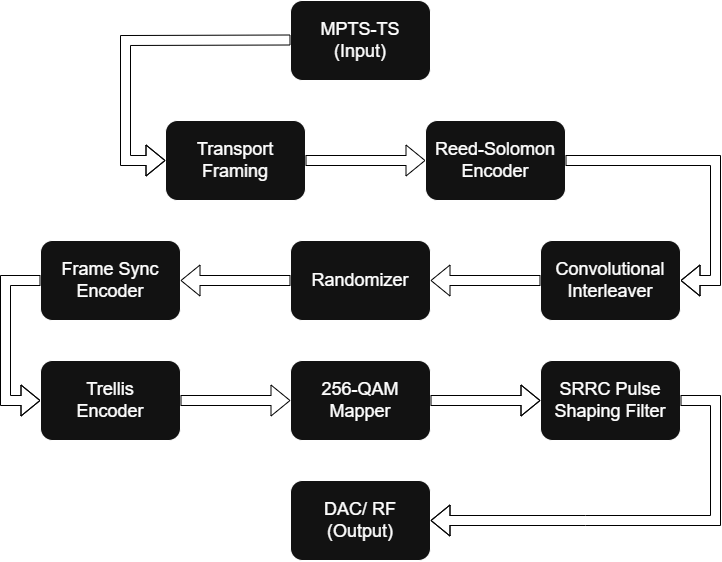
\includegraphics[width=0.64\linewidth]{figures/ch3_j83b_chain.png}
  \caption{J.83B Annex~B downstream processing chain~\cite{ITU_J83}.}
  \label{fig:j83b_chain}
\end{figure}

% ------------------------------------------------------------
\section{DOCSIS 3.0 Downstream Overview}
\label{sec:docsis_overview}

\ac{docsis} 3.0 is the cable industry standard governing broadband
data transmission over \ac{hfc} networks~\cite{DOCSIS3}.
In the downstream direction, from cable headend to \ac{cpe},
\ac{docsis}~3.0 employs \ac{scqam} channels. Each channel
occupies a 6\,MHz bandwidth slot in the North American channel
plan~\cite{SCTE07}.

The downstream channel structure relevant to this work is summarized
in Table~\ref{tab:docsis_params}.

\begin{table}[htbp]
  \caption{DOCSIS 3.0 downstream SC-QAM channel parameters
           (North America)~\cite{DOCSIS3,SCTE07}.}
  \label{tab:docsis_params}
  \centering
  \begin{tabular}{ll}
    \hline
    Parameter           & Value \\
    \hline
    Channel bandwidth   & 6\,MHz \\
    Modulation          & 256-QAM (J.83B Annex~B) \\
    Symbol rate         & 5.360537\,Msym/s \\
    Bits per symbol     & 8 \\
    Information bit rate & 38.81070\,Mbps \\
    % ^ directly from §B.6.1 Table B.3 — citable
    % Raw bit rate (42.884 Mbps = 5.360537×8) and spectral efficiency
    % (≈6.4 bits/s/Hz) are computed values, not stated in standard —
    % omitted from table; include only if derived values section added
    FEC standard        & ITU-T J.83 Annex~B \\
    \hline
  \end{tabular}
\end{table}

A DOCSIS~3.0 downstream system bonds multiple SC-QAM channels to
increase aggregate throughput~\cite{DOCSIS3}.
Each individual channel is independently modulated and passes through
the complete J.83B Annex~B physical layer processing chain described
in this chapter.
The headend \ac{qam} modulator accepts a stream of \ac{mpegts}
packets from the \ac{cmts} and produces
a modulated \ac{rf} signal for distribution over the coaxial plant.
At the subscriber end, a cable modem or set-top box tuner demodulates
the \ac{rf} signal and recovers the \ac{mpegts} byte stream~\cite{DOCSIS3}.

The \ac{qam256} modulation format mandated by J.83B Annex~B~\cite{ITU_J83}
places stringent requirements on the linearity and phase noise
performance of the transmit and receive \ac{rf} chains, and on the
precision of the digital baseband processing blocks described
in the sections that follow~\cite{ITU_J83}.

% ------------------------------------------------------------

\section{J.83B Annex B Standard}
\label{sec:j83b_standard}

ITU-T Recommendation J.83 defines digital multi-programme systems
for television, sound, and data services over cable distribution
networks~\cite{ITU_J83}.
Annex B of the recommendation specifies the physical layer standard
adopted in North America, covering the downstream transmission chain
from MPEG transport stream input to the modulated RF output delivered
over the HFC plant~\cite{ITU_J83,SCTE07}.

The Annex B standard defines a fixed, ordered sequence of processing
stages applied to each MPEG-TS byte stream before modulation.
Table~\ref{tab:j83b_chain_stages} lists each stage in order, together
with the corresponding standard section reference and its role in
the chain.

\begin{table}[htbp]
  \caption{J.83B Annex~B downstream processing chain stages~\cite{ITU_J83}.}
  \label{tab:j83b_chain_stages}
  \centering
  \begin{tabular}{clll}
    \hline
    Stage & Block & Standard Section & Role \\
    \hline
    1 & Transport Framing    & \S B.4     & MPEG-TS packet alignment \\
    2 & Reed-Solomon Encoding & \S B.5.1  & Forward error correction \\
    3 & Convolutional Interleaving & \S B.5.2 & Burst error dispersal \\
    4 & Randomization        & \S B.5.4   & Spectral whitening \\
    5 & Frame Sync Encoding  & \S B.5.3   & Receiver frame lock \\
    6 & Trellis Coding       & \S B.5.5   & Coded modulation \\
    7 & 256-QAM Mapping      & \S B.5.5.5 & Symbol constellation \\
    8 & SRRC Pulse Shaping   & \S B.6.1   & Bandlimited waveform \\
    \hline
  \end{tabular}
\end{table}

Each stage in the chain is described individually in
Sections~\ref{sec:rs_encoding} through~\ref{sec:srrc}.
The remainder of this section provides an overview of the complete
chain and the key system-level parameters that govern its operation.

\paragraph{Transport Framing:}

The chain begins with transport framing, which operates on
MPEG-TS packets of 188 bytes each~\cite{ITU_J83}.
Each packet begins with the standard sync byte \texttt{0x47}~\cite{ITU_J83}.
The framing stage replaces this sync byte in every packet with a
computed parity checksum, derived as the coset of an \ac{fec} parity
check over the preceding 187 payload bytes~\cite{ITU_J83}.
The receiver uses the checksum to detect packet boundaries and
identify packet errors~\cite{ITU_J83}.

\paragraph{Reed-Solomon Encoding:}

\ac{rs} encoding provides the primary \ac{fec}
layer~\cite{ITU_J83}.
The encoder operates on blocks of 122 seven-bit symbols and appends
6 parity symbols to produce a 128-symbol output block~\cite{ITU_J83}.
The code is defined over the Galois field $\mathrm{GF}(2^7)$
and can correct up to 3 symbol errors per block~\cite{ITU_J83}.

\paragraph{Convolutional Interleaving:}

Convolutional interleaving disperses burst errors across multiple
Reed-Solomon blocks so that a single burst affecting several
consecutive bytes at the receiver is spread into correctable
single-byte errors after de-interleaving~\cite{ITU_J83}.
The interleaver is a Forney (convolutional) type with depth
$I = 128$ and increment $J = 1$.

\paragraph{Randomization:}

The randomizer applies a \ac{pn} scrambling sequence to
the interleaved byte stream~\cite{ITU_J83}.
The scrambler operates in $\mathrm{GF}(128)$, initializing its
state to \texttt{0x7F} at each frame boundary and XOR-ing each
7-bit symbol with the \ac{pn} sequence output.
Randomization prevents long runs of identical symbols that would
cause spectral lines in the transmitted signal.

\paragraph{Frame Sync Encoding:}

Frame sync encoding appends a 40-bit trailer to the end of each
FEC frame~\cite{ITU_J83}.
The trailer is packed MSB-first into 7-bit symbols and provides
the receiver with a known pattern for frame boundary detection.

\paragraph{Trellis Coding:}

Trellis coding is applied after frame sync encoding using a 16-state
\ac{bcc} with generator polynomials
$G_1 = 25_8$ and $G_2 = 37_8$~\cite{ITU_J83}.
The \ac{bcc} operates at a punctured rate of 4/5, converting the base
rate 1/2 encoder to produce 5 coded bits for every 4 input
bits~\cite{ITU_J83}.
For \ac{qam256}, the overall trellis coded modulation rate is
19/20~\cite{ITU_J83}, producing 8-bit trellis-coded
words~(C-words) suitable for \ac{qam256} mapping.
A differential precoder is incorporated to resolve phase ambiguity
at the receiver~\cite{ITU_J83}.

\paragraph{256-QAM Symbol Mapping:}

Each 8-bit C-word is mapped to a complex \ac{iq} symbol on the
\ac{qam256} constellation defined by J.83B Figure~B.19~\cite{ITU_J83}.
The output is a stream of complex \ac{iq} samples at the symbol rate
of 5.360537\,Msym/s~\cite{ITU_J83}.
The output is a stream of complex \ac{iq} samples at the symbol rate
of 5.360537\,Msym/s~\cite{ITU_J83}.

\paragraph{SRRC Pulse Shaping:}

The final stage applies \ac{srrc} pulse shaping to the symbol stream.
Table~B.3 of the standard specifies the frequency response as a
\ac{srrc} filter with roll-off $\alpha \approx 0.12$
for \ac{qam256}~\cite{ITU_J83}.
The matched \ac{srrc} filter at the receiver completes the Nyquist
pair, minimizing \ac{isi} at the
sampling instants~\cite{ITU_J83}.
% NOTE: Filter span, samples per symbol, tap count, and output
% sample rate are implementation parameters sourced from
% j83b_srrc_tx.m — NOT stated in the standard.
% These belong in CH-4 (NDA-gated implementation section).
% Do not expand these values in CH-3.

% ------------------------------------------------------------

\section{Reed-Solomon Encoding}
\label{sec:rs_encoding}

\ac{rs} coding forms the outermost layer of the J.83B
\ac{fec} stack, providing block-level error
correction before the data enters the interleaver~\cite{ITU_J83}.
The same \ac{rs} code is used for both 64-QAM and \ac{qam256} operation,
though the \ac{fec} frame format differs between the two modulation
types~\cite{ITU_J83}.

\subsection{Code Definition}

The J.83B \ac{rs} encoder implements a systematic, extended
$(128,\,122)$ \ac{rs} code over the Galois field
$\mathrm{GF}(128) = \mathrm{GF}(2^7)$~\cite{ITU_J83}.
The code corrects up to $t = 3$ symbol errors per \ac{rs} block~\cite{ITU_J83}.
Each symbol is 7 bits wide, matching the field size.

The field is constructed using the primitive polynomial~\cite{ITU_J83}

\begin{equation}
  p(x) = x^7 + x^3 + 1, \quad p(\alpha) = 0
  \label{eq:rs_primitive_poly}
\end{equation}

\noindent where $\alpha$ is the primitive element of
$\mathrm{GF}(128)$.

The generator polynomial is~\cite{ITU_J83}

\begin{equation}
  g(x) = (x - \alpha)(x - \alpha^2)(x - \alpha^3)(x - \alpha^4)
          (x - \alpha^5)
  \label{eq:rs_generator_poly}
\end{equation}

\noindent which expands to

\begin{equation}
  g(x) = x^5 + \alpha^{52}x^4 + \alpha^{116}x^3
             + \alpha^{119}x^2 + \alpha^{61}x + \alpha^{15}
  \label{eq:rs_generator_expanded}
\end{equation}

\subsection{Encoding Procedure}

The encoder accepts a message block of 122 seven-bit symbols,
represented as the message polynomial~\cite{ITU_J83}

\begin{equation}
  m(x) = m_{121}x^{121} + m_{120}x^{120} + \cdots + m_1 x + m_0
  \label{eq:rs_message_poly}
\end{equation}

The message polynomial is multiplied by $x^5$ and divided by
$g(x)$ to produce the remainder~\cite{ITU_J83}

\begin{equation}
  r(x) = r_4 x^4 + r_3 x^3 + r_2 x^2 + r_1 x + r_0
  \label{eq:rs_remainder}
\end{equation}

\noindent These five coefficients constitute the five RS parity
symbols.
The parity symbols are appended to the message to form a 127-symbol code word~\cite{ITU_J83}.

\begin{equation}
  c(x) = m_{121}x^{126} + \cdots + m_0 x^5
        + r_4 x^4 + r_3 x^3 + r_2 x^2 + r_1 x + r_0
  \label{eq:rs_codeword}
\end{equation}

A valid code word has roots at $\alpha^1$ through $\alpha^5$~\cite{ITU_J83}.

\subsection{Extended Parity Symbol}

The J.83B code is extended from $(127,\,121)$ to $(128,\,122)$
by evaluating the 127-symbol code word at the sixth power of
$\alpha$ ~\cite{ITU_J83}

\begin{equation}
  \bar{c} = c(\alpha^6)
  \label{eq:rs_extended_symbol}
\end{equation}

\noindent This extended parity symbol $\bar{c}$ is appended as
the final symbol of the transmitted RS block, yielding the
complete 128-symbol output structure shown in
Table~\ref{tab:rs_block}.

\begin{table}[htbp]
  \caption{J.83B Reed-Solomon block structure~\cite{ITU_J83}.}
  \label{tab:rs_block}
  \centering
  \begin{tabular}{llc}
    \hline
    Symbol positions & Content & Width \\
    \hline
    1 -- 122   & Information symbols ($m_{121}$ \ldots $m_0$) & 7 bits each \\
    123 -- 127 & RS parity symbols ($r_4$ \ldots $r_0$)       & 7 bits each \\
    128        & Extended symbol ($\bar{c} = c(\alpha^6)$)    & 7 bits \\
    \hline
    Total      & 128 symbols                                   & 896 bits \\
    \hline
  \end{tabular}
\end{table}

The parameters of the RS code are summarized in
Table~\ref{tab:rs_params}.

\begin{table}[htbp]
  \caption{J.83B Reed-Solomon code parameters~\cite{ITU_J83}.}
  \label{tab:rs_params}
  \centering
  \begin{tabular}{ll}
    \hline
    Parameter              & Value \\
    \hline
    Code                   & $(128,\,122)$ extended RS \\
    Field                  & $\mathrm{GF}(2^7) = \mathrm{GF}(128)$ \\
    Symbol width           & 7 bits \\
    Information symbols    & 122 per block \\
    Parity symbols         & 5 (RS) $+$ 1 (extended) $= 6$ total \\
    Output block size      & 128 symbols \\
    Correction capability  & $t = 3$ symbol errors per block \\
    \hline
  \end{tabular}
\end{table}

The \ac{rs} encoder output feeds directly into the convolutional
interleaver described in Section~\ref{sec:interleaving}.
The interleaver disperses the 128-symbol \ac{rs} blocks across
multiple frames so that burst channel errors are converted
into correctable single-symbol errors at the \ac{rs} decoder~\cite{ITU_J83}.

% ------------------------------------------------------------
\section{Convolutional Interleaving}
\label{sec:interleaving}

Convolutional interleaving is applied to the \ac{rs}-encoded byte stream
after the encoder and before the randomizer~\cite{ITU_J83}.
Its purpose is to disperse burst channel errors across multiple \ac{rs}
blocks so that a contiguous sequence of corrupted symbols at the receiver
is spread into isolated single-symbol errors after de-interleaving,
keeping the per-block error count within the three-symbol correction
capability of the $(128,\,122)$ \ac{rs} code~\cite{ITU_J83}.

\subsection{Forney Interleaver Structure}

The J.83B interleaver is a Forney convolutional type, operating on
7-bit symbols that match the \ac{rs} field width~\cite{ITU_J83}.
The structure consists of $I$ parallel delay branches, indexed $b = 0, 1, \ldots, I-1$,
with a commutator that cycles through the branches sequentially at the
\ac{rs} symbol rate~\cite{ITU_J83}.
At the start of each \ac{fec} frame the commutator is initialized to
branch~0~\cite{ITU_J83}.

Branch $b$ introduces a delay of~\cite{ITU_J83}

\begin{equation}
  d_b = b \cdot J \quad \text{symbols,} \quad b = 0, 1, \ldots, I-1
  \label{eq:interleaver_branch_delay}
\end{equation}

\noindent so that branch~0 passes symbols with zero delay, branch~1
delays by $J$ symbols, branch~2 by $2J$ symbols, and so on up to
branch $I-1$ which introduces a delay of $(I-1)\cdot J$
symbols.
The de-interleaver at the receiver mirrors this structure, assigning to
branch~$b$ a complementary delay of $(I-1-b)\cdot J$ symbols, so that
the combined round-trip delay is constant at $(I-1)\cdot J$ symbols for
every symbol regardless of which branch it traverses~\cite{ITU_J83}.

The round-trip symbol latency through the interleaver--de-interleaver
pair is therefore

\begin{equation}
  L = I \cdot (I-1) \cdot J \quad \text{symbols.}
  \label{eq:interleaver_latency}
\end{equation}

% [ALT: Block diagram of the J.83B Annex B convolutional interleaver.
%       Input arrives from the Reed-Solomon Encoder as a 7-bit symbol
%       stream and enters an input commutator on the left. The commutator
%       distributes symbols across I parallel delay branches. Branch 1
%       is a direct zero-delay connection. Branch 2 passes through one
%       J-symbol delay register; Branch 3 through two; continuing to
%       Branch I which passes through I-1 registers. An output commutator
%       on the right collects symbols from all branches and passes the
%       interleaved 7-bit stream to the Randomizer.]
\begin{figure}[htbp]
  \centering
  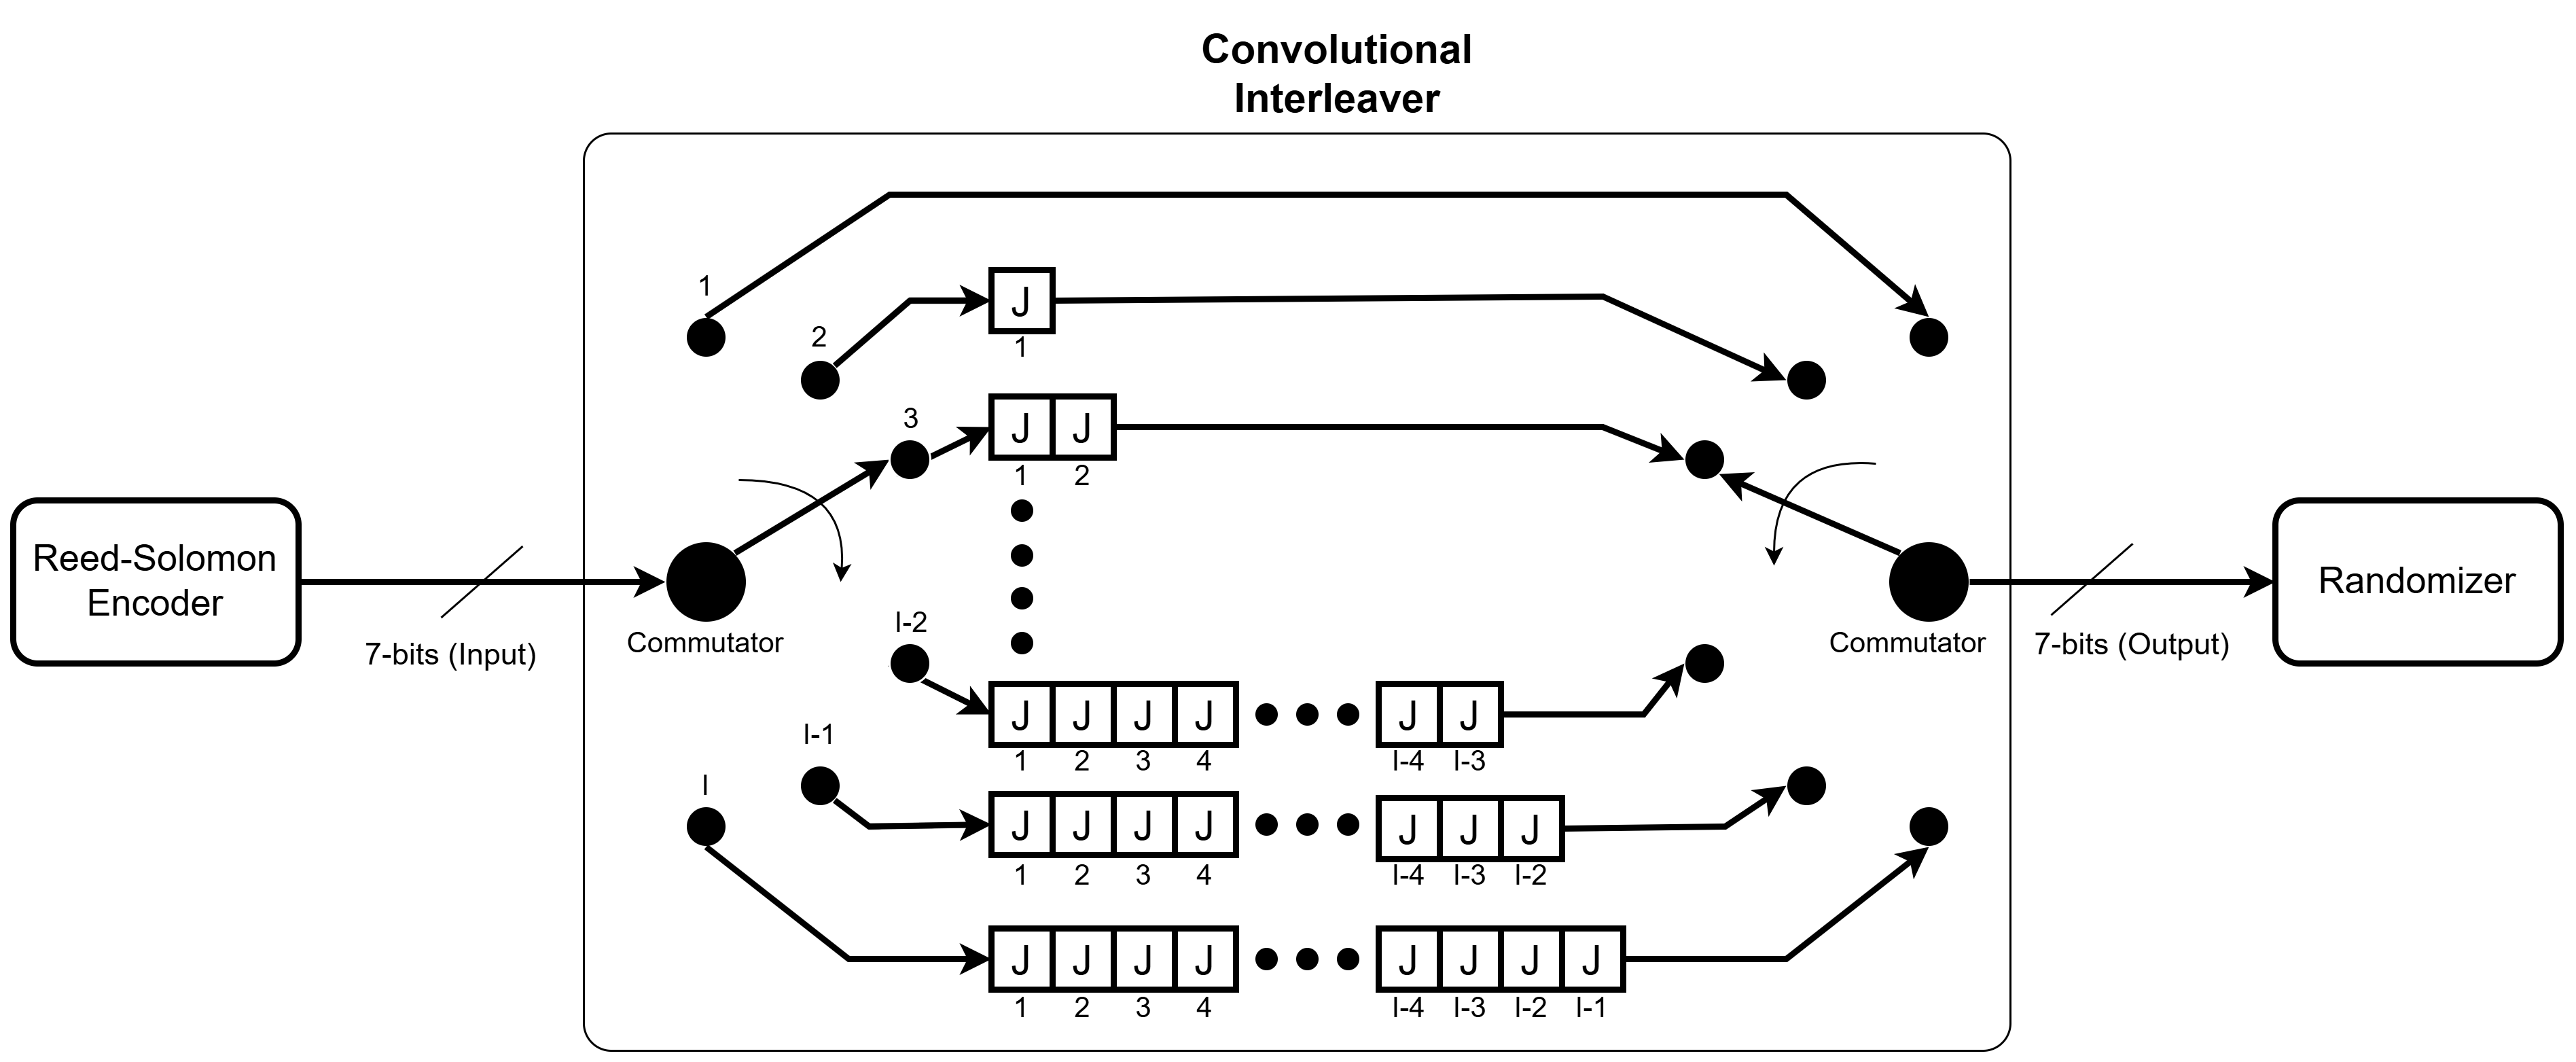
\includegraphics[width=\linewidth]{figures/ch3_interleaver.png}
  \caption{J.83B Annex~B convolutional interleaver structure~\cite{ITU_J83}.
           Branch~$b$ introduces a delay of $b \cdot J$ symbols;
           Branch~1 is a direct connection with zero delay.
           Input commutator cycles at the \ac{rs} symbol rate;
           output feeds the randomizer.}
  \label{fig:interleaver}
\end{figure}

\subsection{Operating Levels and Mode Selection}

J.83B defines two interleaver operating levels~\cite{ITU_J83}.
Level~1 supports a single fixed configuration ($I = 128$, $J = 1$)
and is specified for \ac{docsis} 64-QAM transmission only~\cite{ITU_J83}.
Level~2 extends interleaver support to both 64-QAM and \ac{qam256}
modulation and allows variable interleaving parameters~\cite{ITU_J83}.
A 4-bit in-band control word transmitted during the \ac{fec} frame sync
interval conveys the selected $I$ and $J$ values to the receiver for
the active channel~\cite{ITU_J83}.
Table~\ref{tab:interleaver_modes} lists the defined Level~2 parameter
combinations together with the corresponding burst protection and
latency figures from Table~B.2 of the standard~\cite{ITU_J83}.

\begin{table}[htbp]
  \caption{J.83B Level~2 interleaver parameter options~\cite{ITU_J83}.}
  \label{tab:interleaver_modes}
  \centering
  \begin{tabular}{ccccc}
    \hline
    Control Word & $I$ & $J$ &
      Burst Protection ($\mu$s) &
      Latency, 256-QAM (ms) \\
    \hline
    0001 & 128 & 1 & 66  & 2.8 \\
    0011 &  64 & 2 & 33  & 1.4 \\
    0101 &  32 & 4 & 16  & 0.68 \\
    0111 &  16 & 8 & 8.2 & 0.33 \\
    1001 &   8 & 16 & 4.1 & 0.15 \\
    \hline
  \end{tabular}
\end{table}

The burst protection and latency figures in
Table~\ref{tab:interleaver_modes} exhibit a design trade-off: deeper
interleaving ($I = 128$, $J = 1$) provides greater immunity to
sustained burst noise at the cost of higher end-to-end processing
latency, while shallower configurations reduce latency at the expense
of burst tolerance~\cite{ITU_J83}.

\subsection{Parameters Used in This Work}

This implementation operates in Level~2 mode with control word
\texttt{0001}, corresponding to $I = 128$ branches and increment
$J = 1$ symbol per branch~\cite{ITU_J83}.
This is the maximum-depth configuration and provides the highest burst
protection of the defined Level~2 modes~\cite{ITU_J83}.
Substituting into~\eqref{eq:interleaver_latency}, the round-trip
interleaver--de-interleaver latency is

\begin{equation}
  L = 128 \cdot 127 \cdot 1 = 16{,}256 \quad \text{symbols,}
  \label{eq:interleaver_latency_val}
\end{equation}

\noindent corresponding to a one-way \ac{qam256} channel latency of
2.8\,ms as specified in Table~B.2 of the standard~\cite{ITU_J83}.
The burst protection figure for this mode is
$66\,\mu\mathrm{s}$~\cite{ITU_J83}, which bounds the maximum contiguous
burst duration that the combined interleaver and \ac{rs} decoder can
fully correct.

The interleaved symbol stream feeds directly into the randomizer
described in Section~\ref{sec:randomization}, where a \ac{pn} sequence
is applied for spectral whitening prior to frame sync encoding and
trellis coding~\cite{ITU_J83}.


% ------------------------------------------------------------
\section{Randomization}
\label{sec:randomization}

The randomizer is applied to the interleaved symbol stream after
the convolutional interleaver and before frame sync
encoding~\cite{ITU_J83}.
Its function is to ensure even distribution of symbols across the
\ac{qam256} constellation, which is required for the demodulator
to maintain carrier and timing lock~\cite{ITU_J83}.
Without randomization, long runs of identical symbols produce
spectral lines in the transmitted signal and reduce the effectiveness
of the automatic gain control and phase-locked loop circuits in the
receiver~\cite{ITU_J83}.

\subsection{PN Sequence Generator}

The randomizer XORs each 7-bit interleaved symbol with a
corresponding symbol from a \ac{pn} sequence defined over
$\mathrm{GF}(128) = \mathrm{GF}(2^7)$~\cite{ITU_J83}.
The \ac{pn} sequence is generated by a \ac{lfsr} governed by
the GF(128) recurrence polynomial~\cite{ITU_J83}

\begin{equation}
  f(x) = x^3 + x + \alpha^3
  \label{eq:rand_poly}
\end{equation}

\noindent where $\alpha$ is the primitive element of
$\mathrm{GF}(128)$ satisfying the same reduction polynomial used
by the \ac{rs} encoder~\cite{ITU_J83},

\begin{equation}
  p(x) = x^7 + x^3 + 1.
  \label{eq:rand_reduction_poly}
\end{equation}

The \ac{lfsr} consists of three 7-bit state registers operating
over $\mathrm{GF}(128)$~\cite{ITU_J83}.
At each clock step the register state advances according to
the recurrence in~\eqref{eq:rand_poly}, producing one 7-bit
\ac{pn} output symbol per step.
Each output symbol is bitwise XOR-ed with the corresponding
interleaved data symbol, leaving the 7-bit width of the symbol
stream unchanged~\cite{ITU_J83}.

\subsection{Initialization and Frame Synchronization}

The randomizer is initialized at each \ac{fec} frame
boundary~\cite{ITU_J83}.
Initialization loads all three \ac{lfsr} state registers to the
all-ones state \texttt{0x7F}~\cite{ITU_J83}.
The initialization occurs during the \ac{fec} frame sync trailer
interval; the trailer symbols themselves are therefore not
randomized~\cite{ITU_J83}.
The initialized register state produces the first \ac{pn} output
symbol, which randomizes the first data symbol of the subsequent
\ac{fec} frame~\cite{ITU_J83}.

For \ac{qam256} operation, one \ac{fec} frame consists of
88 \ac{rs} blocks of 128 symbols each, giving a frame data payload
of $88 \times 128 = 11{,}264$ symbols~\cite{ITU_J83}.
The \ac{pn} sequence therefore has a period of 11{,}264 symbols
per frame and is re-initialized at the start of each
frame~\cite{ITU_J83}.

\subsection{Randomizer Parameters}

The randomizer parameters for \ac{qam256} operation are summarized
in Table~\ref{tab:rand_params}.

\begin{table}[htbp]
  \caption{J.83B Annex~B randomizer parameters for
           256-QAM operation~\cite{ITU_J83}.}
  \label{tab:rand_params}
  \centering
  \begin{tabular}{ll}
    \hline
    Parameter              & Value \\
    \hline
    Sequence type          & \ac{lfsr} over $\mathrm{GF}(2^7)$ \\
    Recurrence polynomial  & $f(x) = x^3 + x + \alpha^3$ \\
    Reduction polynomial   & $p(x) = x^7 + x^3 + 1$ \\
    Symbol width           & 7 bits \\
    Initialization state   & \texttt{0x7F} (all ones) \\
    Init trigger           & \ac{fec} frame trailer interval \\
    Operation              & Bitwise XOR per symbol \\
    Sequence period        & $88 \times 128 = 11{,}264$ symbols \\
    \hline
  \end{tabular}
\end{table}

The randomized symbol stream feeds directly into the frame sync
encoder described in Section~\ref{sec:framesync}, where the
\ac{fec} frame trailer is appended and the symbol stream is
unpacked into a serial bit stream for trellis
coding~\cite{ITU_J83}.


% ------------------------------------------------------------
\section{Frame Sync Encoding}
\label{sec:framesync}

Frame sync encoding appends a fixed-pattern trailer to the
randomized symbol stream at the end of each \ac{fec}
frame~\cite{ITU_J83}.
The trailer serves two functions at the receiver: it delineates
the \ac{fec} frame boundary, enabling synchronized \ac{rs}
decoding, de-interleaving, and de-randomization; and it carries
the 4-bit in-band control word that conveys the active interleaver
depth mode to the receiver~\cite{ITU_J83}.
For \ac{qam256}, trellis group boundaries are additionally aligned
to the \ac{fec} frame by the frame sync encoder~\cite{ITU_J83}.

\subsection{FEC Frame Structure}

For \ac{qam256} operation, one \ac{fec} frame consists of 88
\ac{rs} blocks each containing 128 seven-bit symbols~\cite{ITU_J83}.
Each 7-bit symbol is serialized \ac{msb}-first into a contiguous
bit stream, producing~\cite{ITU_J83}

\begin{equation}
  N_\text{data} = 88 \times 128 \times 7 = 78{,}848 \text{ bits}
  \label{eq:fec_data_bits}
\end{equation}

\noindent of data per frame.
The 40-bit sync trailer is appended at the end of the data bit
stream, giving a total frame length of~\cite{ITU_J83}

\begin{equation}
  N_\text{frame} = 78{,}848 + 40 = 78{,}888 \text{ bits}
  \label{eq:fec_frame_bits}
\end{equation}

\noindent which divides exactly into $2076 \times 38$ bits,
corresponding to 2076 trellis groups of 38 input bits
each~\cite{ITU_J83}.
The \ac{rs} block and 7-bit symbol boundaries are aligned to the
end of the \ac{fec} frame~\cite{ITU_J83}.

\begin{table}[htbp]
  \caption{J.83B Annex~B 256-QAM \ac{fec} frame arithmetic~\cite{ITU_J83}.}
  \label{tab:fec_frame_arith}
  \centering
  \begin{tabular}{lr}
    \hline
    Quantity & Value \\
    \hline
    RS blocks per frame           & 88 \\
    Symbols per RS block          & 128 \\
    Bits per symbol (serialized)  & 7 \\
    Data bits per frame           & 78{,}848 \\
    Sync trailer bits             & 40 \\
    Total bits per frame          & 78{,}888 \\
    Trellis groups per frame      & 2{,}076 \\
    Bits per trellis group        & 38 \\
    \hline
  \end{tabular}
\end{table}

\subsection{Sync Trailer Format}

The 40-bit sync trailer is structured as three fields
packed \ac{msb}-first~\cite{ITU_J83}, as shown in
Table~\ref{tab:framesync_trailer}.

\begin{table}[htbp]
  \caption{J.83B Annex~B 256-QAM \ac{fec} frame sync trailer
           structure~\cite{ITU_J83}.}
  \label{tab:framesync_trailer}
  \centering
  \begin{tabular}{clcc}
    \hline
    Field & Content & Width & Value \\
    \hline
    Unique word   & Fixed synchronization pattern & 32 bits
                  & \texttt{71 E8 4D D4}\textsubscript{HEX} \\
    Control word  & Interleaver depth mode        & 4 bits
                  & Level~2 mode code \\
    Reserved      & Set to zero                   & 4 bits
                  & \texttt{0x0} \\
    \hline
    Total         & Sync trailer                  & 40 bits & --- \\
    \hline
  \end{tabular}
\end{table}

The 32-bit unique word \texttt{71 E8 4D D4}\textsubscript{HEX}
is the fixed binary pattern
\begin{center}
\texttt{0111\;0001\;1110\;1000}\\
\texttt{0100\;1101\;1101\;0100}
\end{center}~\cite{ITU_J83}.
The receiver searches for this pattern to detect the \ac{fec}
frame boundary~\cite{ITU_J83}.
The 4-bit control word immediately follows and encodes the active
Level~2 interleaver depth mode as defined in Table~B.2 of the
standard~\cite{ITU_J83}.
The final 4 bits are reserved and set to zero~\cite{ITU_J83}.

The sync trailer is inserted by the encoder and is not
randomized~\cite{ITU_J83}.
The randomizer, described in Section~\ref{sec:randomization}, is
initialized during the trailer interval so that its output is
ready to scramble the first data symbol of the following
frame~\cite{ITU_J83}.

\subsection{Symbol Serialization}

Prior to trellis coding, the frame sync encoder serializes each
7-bit \ac{rs} symbol into individual bits, emitting the most
significant bit first~\cite{ITU_J83}.
The most significant bit of the first \ac{rs} symbol of each
\ac{fec} frame is assigned to the first bit position of the first
non-sync trellis group~\cite{ITU_J83}.
There is no synchronization relationship between the \ac{rs} block
boundaries and \ac{mpegts} packet boundaries; \ac{mpegts}
packet synchronization is obtained independently from \ac{fec}
frame synchronization, keeping the \ac{fec} and transport layers
decoupled~\cite{ITU_J83}.

The serialized bit stream, comprising the 78,848 data bits and the
40-bit trailer (Table~\ref{tab:fec_frame_arith}), feeds directly into the trellis encoder described
in Section~\ref{sec:trellis}~\cite{ITU_J83}.


% ------------------------------------------------------------
\section{Trellis Coding}
\label{sec:trellis}

Trellis coding forms the inner code of the J.83B concatenated
coding scheme~\cite{ITU_J83}.
It introduces redundancy into the transmitted symbol stream to
improve the threshold \ac{snr} by expanding the symbol
constellation without increasing the symbol rate, and is more
precisely termed trellis coded modulation~\cite{ITU_J83}.
For \ac{qam256}, the trellis encoder accepts the serialized bit
stream from the frame sync encoder and produces 8-bit
trellis-coded words, referred to as C-words, that address the
\ac{qam256} constellation mapper~\cite{ITU_J83}.

\subsection{Trellis Group Structure}

The trellis encoder operates on fixed-length groups of input bits
called trellis groups~\cite{ITU_J83}.
For \ac{qam256}, each trellis group contains 38 input bits and
produces 5 output \ac{qam256} symbols, for a total of 40 output
bits per group~\cite{ITU_J83}.

Two types of trellis groups are defined for
\ac{qam256}~\cite{ITU_J83}:

\begin{itemize}
  \item \textbf{Non-sync group:} contains 38 data bits, all
        sourced from the serialized \ac{rs} symbol
        stream~\cite{ITU_J83}.
  \item \textbf{Sync group:} contains 30 data bits and 8 sync
        bits drawn from the \ac{fec} frame sync
        trailer~\cite{ITU_J83}.
        The sync bits occupy only the convolutionally encoded
        bit positions within the group~\cite{ITU_J83}.
\end{itemize}

Since each \ac{fec} frame contains $78{,}888$ bits total (88 \ac{rs}
blocks plus the 40-bit trailer), the frame divides into
$78{,}888 / 38 = 2{,}076$ trellis groups~\cite{ITU_J83}.
Of these, 2{,}071 are non-sync groups and 5 are sync groups;
the 5 sync groups appear at the end of the
frame~\cite{ITU_J83}.

Within each trellis group, the 38 input bits are partitioned by a
data formatter into four streams: the \ac{msb}s of the `A'
symbols, the \ac{msb}s of the `B' symbols, the \ac{lsb}s of
the `A' symbols, and the \ac{lsb}s of the `B'
symbols~\cite{ITU_J83}.
The \ac{msb} streams bypass the convolutional encoder and are
passed directly to the \ac{qam256} mapper
uncoded~\cite{ITU_J83}.
The \ac{lsb} streams are differentially precoded and then
convolutionally encoded before mapping~\cite{ITU_J83}.

\subsection{Binary Convolutional Coder}

The convolutional encoder is a 16-state, non-systematic,
rate~$\frac{1}{2}$ \ac{bcc} with generator
polynomials~\cite{ITU_J83}

\begin{equation}
  G_1(D) = 1 + D^2 + D^4
  \label{eq:bcc_g1}
\end{equation}

\begin{equation}
  G_2(D) = 1 + D + D^2 + D^3 + D^4
  \label{eq:bcc_g2}
\end{equation}

\noindent corresponding to the octal pair $(G_1, G_2) =
(25_8,\,37_8)$~\cite{ITU_J83}.
For each input bit presented to the encoder, two bits are produced
at the output: the $G_1$ output followed by the $G_2$
output~\cite{ITU_J83}.
The commutator is initialized to the $G_1$ position at the
beginning of each trellis group~\cite{ITU_J83}.

Four input bits per trellis group produce 8 convolutionally
encoded bits~\cite{ITU_J83}.
These 8 bits are reduced to 5 by a puncture matrix applied
over the 4-input block~\cite{ITU_J83}

\begin{equation}
  \begin{bmatrix} P_1 \\ P_2 \end{bmatrix}
  =
  \begin{bmatrix} 0 & 0 & 0 & 1 \\ 1 & 1 & 1 & 1 \end{bmatrix}
  \label{eq:bcc_puncture}
\end{equation}

\noindent where $1$ denotes transmission and $0$ denotes suppression.
The puncture matrix converts the rate~$\frac{1}{2}$ encoder to
rate~$\frac{4}{5}$, retaining 5 of the 8 encoded bits per trellis
group~\cite{ITU_J83}.
Two independent \ac{bcc} instances operate in parallel: one
encodes the `A' \ac{lsb} stream producing outputs $U_1$ through
$U_5$, and one encodes the `B' \ac{lsb} stream producing outputs
$V_1$ through $V_5$~\cite{ITU_J83}.

\subsection{Differential Precoder}

Prior to convolutional encoding, the \ac{lsb} streams pass
through a differential precoder that provides 90° rotational
invariance~\cite{ITU_J83}.
Rotational invariance allows the receiver to recover data
correctly following a carrier phase slip without requiring
\ac{fec} resynchronization, since information is carried by the
change in phase rather than its absolute
value~\cite{ITU_J83}.
For \ac{qam256}, the 4th and 8th bits of each C-word are
differentially encoded, corresponding to positions $C_4$ and $C_0$
in the constellation labelling of Figure~B.19 of the
standard~\cite{ITU_J83}.

The differential precoder update equations
are~\cite{ITU_J83}

\begin{equation}
  x_J = W_J \oplus x_{J-1} \oplus Z_J \cdot (x_{J-1} \oplus Y_{J-1})
  \label{eq:precode_x}
\end{equation}

\begin{equation}
  Y_J = Z_J \oplus W_J \oplus Y_{J-1} \oplus Z_J \cdot (x_{J-1} \oplus Y_{J-1})
  \label{eq:precode_y}
\end{equation}

\noindent where $W_J$ and $Z_J$ are the two input bits at step
$J$, $x_J$ and $Y_J$ are the two precoded output bits, $\oplus$
denotes XOR, and $(\cdot)$ denotes the AND
operation~\cite{ITU_J83}.

\subsection{Overall Code Rate and Output}

Each trellis group produces 40 output bits from 38 input bits,
giving an overall trellis coded modulation rate
of~\cite{ITU_J83}

\begin{equation}
  R_\text{TCM} = \frac{38}{40} = \frac{19}{20}
  \label{eq:trellis_rate}
\end{equation}

The 40 output bits per trellis group are packed into 5 eight-bit
C-words, each of which addresses one symbol position in the
\ac{qam256} constellation~\cite{ITU_J83}.
The trellis encoder output feeds directly into the \ac{qam256}
symbol mapper described in
Section~\ref{sec:qam256}~\cite{ITU_J83}.

The trellis coding parameters for \ac{qam256} operation are
summarized in Table~\ref{tab:trellis_params}.

\begin{table}[htbp]
  \caption{J.83B Annex~B trellis coding parameters for
           256-QAM operation~\cite{ITU_J83}.}
  \label{tab:trellis_params}
  \centering
  \begin{tabular}{ll}
    \hline
    Parameter                  & Value \\
    \hline
    Encoder type               & 16-state non-systematic \ac{bcc} \\
    Generator polynomials      & $G_1 = 25_8,\; G_2 = 37_8$ \\
    Base code rate             & $1/2$ \\
    Puncture matrix            & $[P_1;\,P_2] = [0001;\,1111]$ \\
    Punctured code rate        & $4/5$ \\
    Overall \ac{tcm} rate     & $19/20$ \\
    Input bits per group       & 38 \\
    Output symbols per group   & 5 \\
    Output bits per group      & 40 \\
    Trellis groups per frame   & 2{,}076 (2{,}071 non-sync $+$ 5 sync) \\
    C-word width               & 8 bits \\
    \hline
  \end{tabular}
\end{table}


% ------------------------------------------------------------
\section{256-QAM Symbol Mapping}
\label{sec:qam256}

The \ac{qam256} symbol mapper converts the 8-bit C-words
produced by the trellis encoder into complex \ac{iq} baseband
symbols for transmission~\cite{ITU_J83}.
Each C-word addresses a look-up table that returns the complex
symbol coordinates corresponding to that C-word's position on the
\ac{qam256} constellation defined by Figure~B.19 of the
standard~\cite{ITU_J83}.
The mapper output is a stream of complex \ac{iq} samples at the
J.83B symbol rate of 5.360537\,Msym/s, which feeds directly into
the \ac{srrc} pulse shaping filter described in
Section~\ref{sec:srrc}~\cite{ITU_J83}.

\subsection{Constellation Geometry}

The J.83B \ac{qam256} constellation is a square, 256-point array
arranged on a $16 \times 16$ grid in the \ac{iq}
plane~\cite{ITU_J83}.
The in-phase and quadrature axes each carry 16 equally spaced
amplitude levels at odd integer values $\{-15,\,-13,\,\ldots,\,-1,
\,+1,\,\ldots,\,+13,\,+15\}$, giving $16^2 = 256$ distinct symbol
positions~\cite{ITU_J83}.
The constellation is symmetric about both the I and Q axes, and
the minimum Euclidean distance between adjacent symbols is
uniform across the grid~\cite{ITU_J83}.

\subsection{C-Word to Symbol Mapping}

The trellis encoder delivers the coded and uncoded 4-bit `A' and
`B' streams to the mapper, which concatenates them into a single
8-bit C-word with C-bit ordering $C_7 C_6 C_5 C_4\,C_3 C_2 C_1
C_0$ where $C_7$ is the \ac{msb}~\cite{ITU_J83}.
The 8-bit C-word takes values in the range $0$\,--\,$255$ and
uniquely identifies one of the 256 constellation points via the
look-up table defined by Figure~B.19 of the standard~\cite{ITU_J83}.
The mapping is a bijection: every C-word value corresponds to
exactly one symbol position, and every symbol position is
addressed by exactly one C-word~\cite{ITU_J83}.

The differential precoder bits $C_4$ and $C_0$ occupy
the two differentially encoded positions within the C-word, as
noted in Section~\ref{sec:trellis}~\cite{ITU_J83}.
The remaining six C-word bits are passed through uncoded and
carry the \ac{msb} streams directly from the data
formatter~\cite{ITU_J83}.

% NOTE: Gray coding is NOT explicitly stated in the J.83B standard text.
% J83B_FACTS.md flags: "verify from Figure B.19 constellation pattern."
% Do NOT claim Gray coding in this section without Figure B.19 verification.
% This note is for the author; remove before submission.

\subsection{IQ Output and Symbol Rate}

The mapper output is a stream of complex baseband samples of
the form $s_k = I_k + j Q_k$, where $I_k$ and $Q_k$ are the
in-phase and quadrature coordinates of the $k$-th mapped
symbol~\cite{ITU_J83}.
One complex sample is produced per C-word, at a rate equal to the
J.83B symbol rate of 5.360537\,Msym/s~\cite{ITU_J83}.

The \ac{qam256} symbol mapping parameters are summarized in
Table~\ref{tab:qam256_params}.

\begin{table}[htbp]
  \caption{J.83B Annex~B 256-QAM symbol mapping
           parameters~\cite{ITU_J83}.}
  \label{tab:qam256_params}
  \centering
  \begin{tabular}{ll}
    \hline
    Parameter              & Value \\
    \hline
    Constellation          & Square 256-QAM \\
    Grid size              & $16 \times 16$ \\
    Symbol positions       & 256 \\
    I/Q amplitude levels   & $\{-15,\,-13,\,\ldots,\,+13,\,+15\}$ \\
    Input C-word width     & 8 bits ($C_7$\,--\,$C_0$) \\
    Mapping definition     & Figure~B.19, ITU-T J.83 Annex~B \\
    Implementation         & Look-up table (bijection) \\
    Output                 & Complex \ac{iq} symbol stream \\
    Symbol rate            & 5.360537\,Msym/s \\
    \hline
  \end{tabular}
\end{table}


% ------------------------------------------------------------
\section{SRRC Pulse Shaping}
\label{sec:srrc}

\ac{srrc} pulse shaping is the final stage of the J.83B transmit
processing chain, applied to the complex \ac{iq} symbol stream
after \ac{qam256} mapping~\cite{ITU_J83}.
The \ac{srrc} filter bandlimits the symbol stream to fit within
the 6\,MHz channel allocation, controls the spectral shape of the
transmitted signal, and forms one half of the matched filter pair
that minimizes \ac{isi} at the receiver sampling
instants~\cite{ITU_J83}.
The standard refers to this filter as a square-root raised cosine
filter in Table~B.3 and as a Root-Nyquist filter in
\S B.6.2~\cite{ITU_J83}.

\subsection{Nyquist Matched Filter Pair}

The J.83B pulse shaping scheme employs a matched \ac{srrc} filter
pair: an \ac{srrc} filter at the transmitter and an identical
\ac{srrc} filter at the receiver~\cite{ITU_J83}.
The cascade of the transmit and receive \ac{srrc} filters satisfies
the Nyquist \ac{isi} criterion~\cite{proakis_dsp}, producing a
raised cosine overall frequency response

\begin{equation}
  H_\text{RC}(f) = H_\text{TX}(f) \cdot H_\text{RX}(f)
                 = \left| H_\text{SRRC}(f) \right|^2
  \label{eq:srrc_matched}
\end{equation}

\noindent where $H_\text{TX}(f) = H_\text{RX}(f) = H_\text{SRRC}(f)$
are the identical transmit and receive \ac{srrc} frequency
responses~\cite{proakis_dsp}.
The raised cosine response $H_\text{RC}(f)$ has zero crossings at
all non-zero integer multiples of the symbol period $T_s =
1/f_\text{sym}$, ensuring zero \ac{isi} at the receiver sampling
instants when the channel is ideal~\cite{proakis_dsp}.

The \ac{srrc} frequency response is~\cite{proakis_dsp}

\begin{equation}
  H_\text{SRRC}(f) =
  \begin{cases}
    \sqrt{T_s}, & |f| \leq \dfrac{1-\alpha}{2T_s} \\[6pt]
    \sqrt{\dfrac{T_s}{2}\!\left[1 + \cos\!\left(
      \dfrac{\pi T_s}{\alpha}\!\left(|f| - \dfrac{1-\alpha}{2T_s}
      \right)\right)\right]}, &
      \dfrac{1-\alpha}{2T_s} < |f| \leq \dfrac{1+\alpha}{2T_s} \\[6pt]
    0, & |f| > \dfrac{1+\alpha}{2T_s}
  \end{cases}
  \label{eq:srrc_response}
\end{equation}

\noindent where $f_\text{sym} = 1/T_s$ is the symbol rate and
$\alpha$ is the roll-off factor~\cite{proakis_dsp}.
The one-sided occupied bandwidth of the filtered signal is
$(1+\alpha)/(2T_s)$, so the total double-sided bandwidth is
$(1+\alpha) \cdot f_\text{sym}$~\cite{proakis_dsp}.

\subsection{J.83B Filter Specification}

For \ac{qam256}, Table~B.3 of the standard specifies the transmit
filter as a square-root raised cosine with roll-off
factor~\cite{ITU_J83}

\begin{equation}
  \alpha = 0.12 \quad \text{(256-QAM)}
  \label{eq:srrc_alpha}
\end{equation}

\noindent and the symbol rate~\cite{ITU_J83}

\begin{equation}
  f_\text{sym} = 5.360537\,\text{Msym/s} \pm 5\,\text{ppm.}
  \label{eq:srrc_symrate}
\end{equation}

Substituting into the bandwidth expression, the double-sided
occupied bandwidth of the J.83B \ac{qam256} channel
is~\cite{ITU_J83}

\begin{equation}
  B = (1 + \alpha) \cdot f_\text{sym}
    = 1.12 \times 5.360537 \approx 6.004\,\text{MHz}
  \label{eq:srrc_bw}
\end{equation}

\noindent which fits within the 6\,MHz channel slot defined by the
North American channel plan~\cite{ITU_J83,SCTE07}.

\subsection{RF Output Signal Model}

The \ac{rf} modulated output signal is formed by modulating the
\ac{srrc}-filtered baseband \ac{iq} components onto the carrier
frequency $f_c$~\cite{ITU_J83}

\begin{equation}
  s(t) = I(t)\cos(2\pi f_c t) - Q(t)\sin(2\pi f_c t)
  \label{eq:rf_output}
\end{equation}

\noindent where $I(t)$ and $Q(t)$ are the Root-Nyquist filtered
baseband in-phase and quadrature components of the constellation
symbols, and $f_c$ is the \ac{rf} carrier
frequency~\cite{ITU_J83}.

The J.83B \ac{srrc} pulse shaping parameters are summarized in
Table~\ref{tab:srrc_params}.
Filter implementation parameters - including filter span, samples
per symbol, tap count, and output sample rate - are
implementation-specific design choices and are described in
Chapter~4.

\begin{table}[htbp]
  \caption{J.83B Annex~B \ac{srrc} pulse shaping parameters for
           256-QAM operation (standard-sourced)~\cite{ITU_J83}.}
  \label{tab:srrc_params}
  \centering
  \begin{tabular}{ll}
    \hline
    Parameter              & Value \\
    \hline
    Filter type            & Square-root raised cosine (\ac{srrc}) \\
    Standard reference     & \S B.6.1 Table~B.3, \S B.6.2 \\
    Roll-off factor $\alpha$ & 0.12 (256-QAM) \\
    Symbol rate input      & 5.360537\,Msym/s $\pm$ 5\,ppm \\
    Occupied bandwidth     & $\approx 6.004$\,MHz \\
    Channel slot           & 6\,MHz \\
    Matched filter         & TX \ac{srrc} $\times$ RX \ac{srrc} $=$ RC \\
    \ac{isi} at sampling  & Zero (Nyquist criterion, ideal channel) \\
    \hline
  \end{tabular}
\end{table}